\documentclass{article}
\usepackage[utf8]{inputenc}
\usepackage{mathtools}
\usepackage{enumerate}
\usepackage{pgfplots}
\usepackage{tikz}
\usepackage{amsthm}
\usepackage{amssymb}

\title{Sistemas expertos probabilísticos}
\author{Anabel Gómez Ríos\\
        Jacinto Carrasco Castillo}
\date{Mayo 2016}

\begin{document}

\maketitle

\section{Introducción}
En clase hemos visto sistemas expertos basados en reglas del tipo \textbf{SI} \textit{condición} \textbf{ENTONCES} \textit{acción} (donde tanto en \textit{condición} como en \textit{acción} pueden aparecer expresiones lógicas compuestas). En estos sistemas se comprueba si \textit{condición} es cierta o no y, en caso de serlo, se lleva a cabo \textit{acción}.\\

Este tipo de sistemas son muy útiles y muy utilizados por su simplicidad y el parecido con el razonamiento humano, pero presentan varios inconvenientes:
\begin{enumerate}
    \item Mantener la coherencia entre las reglas de la base de conocimiento. Pueden aparecer dos tipos de problemas: encadenamientos infinitos, cuando aparecen reglas del tipo \textit{Si A entonces B} junto con \textit{Si B entonces A} y problemas de ampliación en la base de conocimiento cuando hay que realizar una actualización y para mantener la coherencia la base de datos se hace innecesariamente grande, llegando incluso a ser mejor reconstruirla de nuevo.
    \item Dificultades para retractarse de anteriores conclusiones, provocado principalmente por el carácter modular y monótono de estos sistemas, ya que cuando se cumple la condición de una regla, se da la acción sin tener en cuenta el resto del conocimiento. 
    \item Opacidad: Al tener que dividir el conocimiento en pequeñas reglas, se pierde perspectiva global del problema tratado.
    \item Ineficiencia provocada por la continua comprobación de las reglas en cada iteración.
\end{enumerate}

Sin embargo el principal problema es que cuando se trabaja con problemas reales y conocimiento humano en la mayoría de los casos hay inherente incertidumbre bien en el conocimiento, es decir, en cómo se ha obtenido el conocimiento, o bien en el conjunto de datos, es decir, si los datos no se han determinado de forma precisa o faltan datos.\\
Normalmente, las evidencias que tenemos sobre un hecho no nos permiten deducir con seguridad las conclusiones o la negación de las mismas, pero sí nos permiten dar mayor credibilidad a una sentencia. Por esto, si queremos diseñar un sistema experto capaz de obtener las mismas conclusiones que un experto humano, tenemos darle la capacidad de trabajar con incertidumbre.

\section{Ejemplo de sistema experto Probabilístico:\\ MYCIN}
MYCIN fue el primer sistema experto que consideró conocimiento incierto. En este sistema, una regla \textbf{Si} A \textbf{Entonces} B se representaba $A \overset{m}{\rightarrow}B$, expresando que si se conoce $A$, entonces se puede actualizar la certeza de $B$ en cierta cantidad, en función de la fuerza de la regla, $m$. El valor $m$ se denomina factor de certeza de la regla y toma valores en el intervalo $[-1,1]$.\\

Supongamos el siguiente ejemplo:
\[A \overset{m_1=0.8}{\longrightarrow} B ; B\ y\ C \overset{m_2=0.7}{\longrightarrow} D
\]
y observamos $A$ (y por tanto la certeza de $A$, que vamos a representar $Ctz(A)$ es 1) y la certeza sobre $C$ es 0.6. Entonces, nuestra creencia de $B$ se actualiza a un valor 0.8, $Ctz(B)=0.8$ y tenemos que actualizar la certeza sobre $D$. En estos casos, MYCIN calcula el valor de certeza para la sentencia $B\ y \ C$ como una función de las certezas de $A$ y $B$: $Ctz(B\ y\ C) = min{0.8,0.6}=0.6$ y por tanto $Ctz(D)=0.6*0.7=0.42$.\\
%?
Después veremos mecanismos de propagación que permiten trabajar con sistemas más complejos.

\section{Problemas de los sistemas expertos con incertidumbre}
\begin{enumerate}
    \item Aparecen problemas cuando tratamos de utilizar un razonamiento en los dos sentidos, ya que puede llevar a ciclos indefinidos (por ejemplo con las reglas \textit{\textbf{Si} hay humo \textbf{Entonces} es más creíble que haya fuego} y \textit{\textbf{Si} hay fuego \textbf{Entonces} hay humo}.
    \item No tratan de forma adecuada las fuentes de información dependientes, ya que cuando se dispara una regla, el peso que se asigna a la conclusión depende sólo del peso de las premisas, no de dónde vienen, y puede que vengan de una única fuente que ha seguido diferentes caminos o de fuentes independientes (esto debería influir en la certeza, ya que nos está llegando información de dos sitios distintos).
\end{enumerate}

\section{Comparación con los sistemas expertos basados en reglas}

\subsection{Base de conocimiento}

El conocimiento de un sistema experto basado en reglas consiste en los hechos y el conjunto de reglas. En un sistema experto basado en probabilidad, el conocimiento viene dado por un espacio de probabilidad que incluye las variables, sus posibles valores y su función de probabilidad conjunta. En ambos sistemas los datos consisten en la evidencia asociada a los casos a analizar.\\
Las diferencias también se encuentran en la dificultad para implementar la base de conocimientos. Mientras que en el sistema experto basado en reglas ``sólo'' necesitamos usar elementos como objetos, conjunto de valores, premisas, conclusiones y reglas; en los sistemas expertos basados en probabilidad el conocimiento puede ser mucho más extenso. Por contra, son necesarios numerosos parámetros, lo que dificulta su definición.

\subsection{Motor de inferencia}

El motor de inferencia también es más sencillo de implementar en los sistemas expertos basados en reglas, ya que obtenemos las conclusiones a partir de los hechos aplicando estrategias de inferencia como \textit{modus ponens}, \textit{modus tollens} y encadenamiento de reglas. En los sistemas expertos basados en probabilidad, el motor de inferencia se basa en la evaluación de las probabilidades condicionales, utilizando uno o varios métodos propuestos por diferentes tipos de sistemas expertos probabilísticos. El grado de dificultad de implementar un motor de inferencia probabilístico será mayor y crece si usamos modelos de dependencia generales en detrimento de modelos de independencia.

\subsection{Subsistema de explicación}

La explicación en el sistema basado en regla viene dada por las reglas que se han activado para determinar esa conclusión en cada momento. En el caso probabilístico la información sobre qué variables influyen en otras está codificada en la función de probabilidad conjunta, lo que hace que la explicación se base en los valores relativos de las probabilidades condicionales que miden los grados de dependencia. Una comparación de las probabilidades condicionales para diferentes conjuntos de evidencia permite analizar sus efectos en las conclusiones.

\subsection{Subsistema de aprendizaje}

En los sistemas expertos basados en reglas, el aprendizaje consiste en incorporar nuevos objetos, valores factibles para los objetos, nuevas reglas o modificaciones de los conjuntos existentes, valores posibles o reglase. En los sistemas expertos probabilísticos, consiste en incorporar o modificar la estructura del espacio de probabilidad: variables, posibles valores o parámetros.

\section{Teoría de la Probabilidad}
Vamos a ver algunas nociones básicas de probabilidad que serán de utilidad para trabajar con este tipo de sistemas.

\subsection{Probabilidad de un suceso}



\section{Redes bayesianas}

Las redes bayesianas son uno de los modelos con más importancia en los sistemas expertos probabilísticos. Gráficamente consisten en un grafo dirigido acíclico, donde los nodos son variables del problema a resolver. Las redes bayesianas permiten representar dos aspectos del conocimiento:

\begin{enumerate}
\item \textbf{Cualitativo}: Relaciones de dependencia e independencia entre variables. Dos variables conectadas por un arco estarán relacionadas.
\item \textbf{Cuantitativo}: Fuerza con la que nos creemos las relaciones de relevancia o dependencia.
\end{enumerate} 

Usaremos la representación mediante grafos para representar la dependencia, por

\begin{center}
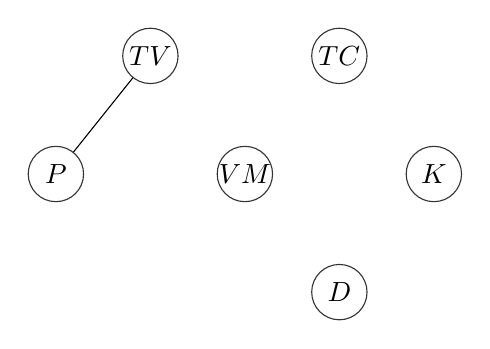
\begin{tikzpicture}[y=.3cm, x=.3cm,font=\normalsize]

\draw[->] (4,10) edge (0,5);

\filldraw[fill=white!0,draw=black!80] (0,5) circle (10pt) node[] {$P$};
\filldraw[fill=white!0,draw=black!80] (4,10) circle (10pt) node[] {$TV$};
\filldraw[fill=white!0,draw=black!80] (8,5) circle (10pt) node[] {$VM$};
\filldraw[fill=white!0,draw=black!80] (12,10) circle (10pt) node[] {$TC$};
\filldraw[fill=white!0,draw=black!80] (12,0) circle (10pt) node[] {$D$};
\filldraw[fill=white!0,draw=black!80] (16,5) circle (10pt) node[] {$K$};

\end{tikzpicture}
\end{center}

\section{Cadenas de Markov}

\section{Métodos de propagación}

%¿?
\section{Modelos en el campo de la medicina}

\section{Bibliografía}


\end{document}
